\documentclass[11pt]{article}
\usepackage{hyperref}
\hypersetup{pdfborder=0 0 0}
\usepackage{setspace}
\usepackage[utf8]{inputenc}
\usepackage[french]{babel}
\usepackage[T1]{fontenc}
\usepackage{amsmath}
\usepackage{amssymb}
\usepackage{xcolor}
\usepackage{graphicx}
\usepackage{enumitem}
\newcommand{\hsp}{\hspace{20pt}}
\newcommand{\HRule}{\rule{\linewidth}{0.5mm}}
\usepackage{float}
\usepackage{comment}
\newcommand{\betamco}{\widehat{\beta}}
\usepackage{eurosym}
\usepackage{enumitem}
\usepackage{geometry}
%\geometry{top=3cm, bottom=2.5cm, left=3.6cm, right=3.6cm}


\begin{document}
\begin{titlepage}
    \begin{sffamily}
    \begin{center}
    \includegraphics[scale=0.5]{pops.png}~\\[1.5cm]
    \HRule \\[0.4cm]
    { \huge \bfseries Projet Python \\ Sujet 5
    \\[0.4cm] }
    \HRule \\[2cm]
    \includegraphics[scale=0.4]{su.png}
    \\[1.4cm]
    \begin{minipage}{0.4\textwidth}
    \begin{flushleft} \large
    \textsc{Aminata Traore}\\
    \textsc{Maxime Lafont Trevisan}\\
    \textsc{Florian Guily}\\
    \textsc{Thomas Halouis}  \\
    Promo 2019/2020\\
    \end{flushleft}
    \end{minipage}
    \begin{minipage}{0.4\textwidth}
    \begin{flushright} \large
    \emph{ Mme.  \textsc{Comte}} \\
    \emph{ M.  \textsc{Ouzia}}
    \end{flushright}
    \end{minipage}
    \vfill
    {\large \today}
    \end{center}
    \end{sffamily}
\end{titlepage}
\tableofcontents
\newpage
\section{Introduction}
Le système d'équations suivant est appelé équations de compétition de Lotka-Volterra. \begin{center}
\[
\left\{
\begin{array}{r c}
N_1'(t) = N_1 \big( r_1 - \cfrac{r_1N_1}{K_1} - \cfrac{\alpha r_1N_2}{K_1} + \gamma N_2\big) & \\
N_2'(t) = N_2 \big( r_2 - \cfrac{r_2N_2}{K_2} - \cfrac{\beta r_2N_1}{K_2} - \delta N_1\big) &
\end{array}
\right.
\]
\end{center}

C'est un modèle simple de dynamique des populations entre deux espèces. Pour une meilleure compréhension de ce rapport, nous allons vous expliquer à quoi chaque paramètre correspond. 
$N_i$ représente le nombre d’individus de la -$i$ème espèce, $K_i$ est la capacité biotique du milieu c'est à dire le nombre d’individus de la -$i$ème espèce que peut nourrir le milieu, $r_i $ est le taux de
croissance  de la -$i$ème espèce, $\alpha$ l’influence de la deuxième espèce sur la première espèce, $\beta$ l’influence de la première
espèce sur la deuxième espèce, $\gamma$ et $\delta$ sont des facteurs de conversion.
A l'aide de ces équations,il est possible de modéliser plusieurs systèmes d'interactions entre deux espèces.
\section{Analyse mathématique}
\subsection{Analyse de la stabilité}
Pour trouver les points singuliers on résout le système suivant : 
\[
\left\{
\begin{array}{r c}

N_1'(t) = N_1 \big( r_1 - \cfrac{r_1N_1}{K_1} - \cfrac{\alpha r_1N_2}{K_1} + \gamma N_2\big) & = 0 \\
N_2'(t) = N_2 \big( r_2 - \cfrac{r_2N_2}{K_2} - \cfrac{\beta r_2N_1}{K_2} - \delta N_1\big) & = 0
\end{array}
\right.
\]


Il faut distinguer plusieurs cas de figures. En effet, deux espèces peuvent cohabiter dans un milieu de plusieurs manières (Indifférence totale,proies-prédateurs,symbiose,parasitage).
\subsection{Espèces indifférentes}

Les deux espèces vivent dans le même milieu mais sans aucun contact et influence l'une sur l'autre. Donc $\alpha=\beta=\gamma=\delta=0$. Dans cette situation nous étudierons des espèces avec des taux de croissance positifs. En effet, dans le cas contraire, elles disparaîtraient car aucun autre paramètre que leur croissance intrinsèque n'influe sur elles. On va donc considérer dans la suite que $r_1 > 0$ et $r_2 > 0$.

Nous allons calculer les points d'équilibres du système avec ces conditions puis nous les retrouverons à l'aide du portrait de phase du système.
\[
\left\{
\begin{array}{r c}

N_1'(t) = N_1r_1 \big( 1 - \cfrac{N_1}{K_1} \big) & = 0 \\
N_2'(t) = N_2r_2 \big( 1 - \cfrac{N_2}{K_2} \big)  & = 0
\end{array}
\right.
\]

$(0,0),(K_1,K_2)(K_1,0),(0,K_2)$ sont des points d'équilibres.
Pour déterminer la stabilité de ces points nous allons injecter ces couples dans la matrice jacobienne du système et regarder la partie réelle des valeurs propres du systèmes. Si elles sont positives le point est instable, si elles sont négatives le point est asymptotiquement stable.
\begin{center}
\begin{math}
J = 
\begin{pmatrix} 
r_1 - \cfrac{2r_1N_1}{K_1}  & 0 \\
0   & r_2 - \cfrac{2r_2N_2}{K_2}   \\
\end{pmatrix}
\end{math}
\end{center}
Pour le couple $(0,0)$ les valeurs propres sont $r_1$ et $r_2$. Donc ce point est instable. \\
Pour le couple $(K_1,K_2)$ les valeurs propres sont $r_1(\frac{1}{K_1} - 2) $et  $r_2(\frac{1}{K_2} - 2) $ donc
$(K_1,K_2)$ est stable et attractif (asymptotiquement stable) si et seulement si $K_1$ et $K_2$ sont supérieurs à $\frac{1}{2}$.\\
Pour le couple $(K_1,0)$ les valeurs propres sont $-r_1 $ et  $r_2$ donc 
$(K_1,0)$ est instable.\\
Pour le couple $(0,K_2)$ les valeurs propres sont $r_1 $ et  $-r_2$ donc 
$(0,K_2)$ instable.

Pour vérifier ces calculs, nous allons tracer le portrait de phase du système.
\begin{center}
\begin{figure}[H]
    \centering
    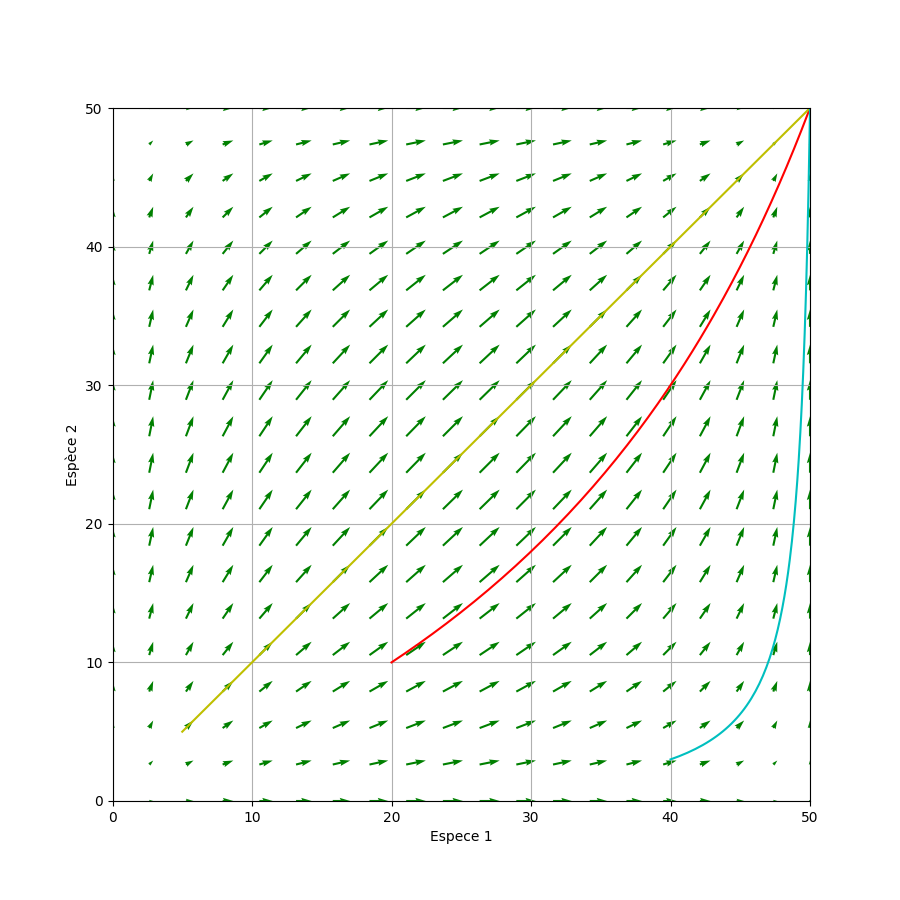
\includegraphics[scale = 0.6]{abnul.png}
    \caption{Croissance de deux espèces à partir de populations de départ différentes}
    \label{0}
\end{figure}
\end{center}

En observant le portrait de phase ci-dessus, on remarque que malgré des conditions initiales différentes, les trois trajectoires convergent vers le point $(50,50)$. Ce point correspond aux valeurs de $K_1$ et $K_2$ utilisées afin de tracer cet exemple. On avait précédemment calculé que le point $(K_1,K_2)$ était asymptotiquement stable. On retrouve bien ce résultat ce qui confirme la théorie.
\subsection{Espèces en compétitions : $\alpha,\beta \ne 0$ \& $\gamma,\delta = 0$ }
En rajoutant les paramètres $\alpha,\beta$ au système il est possible de complexifier le système pour modéliser plus de situations. En effet, en jouant sur le taux de croissance des deux espèces et la capacité biotique du système il est possible de modéliser un système proie prédateurs ou tout du moins une cohabitation auto-régulée entre deux espèces.
\[
\left\{
\begin{array}{r c}

N_1'(t) = N_1 \big( r_1 - \cfrac{r_1N_1}{K_1} - \cfrac{\alpha r_1N_2}{K_1}) & = 0 \\
N_2'(t) = N_2 \big( r_2 - \cfrac{r_2N_2}{K_2} - \cfrac{\beta r_2N_1}{K_2}) & = 0
\end{array}
\right.
\]
Les points d'équilibres sont $(0,0)$,$(K_1,0),(0,K_2)$ et $(K_1 - \alpha \dfrac{K_2-\beta K_1}{1 -\alpha \beta},\dfrac{K_2-\beta K_1}{1 -\alpha \beta})$ avec $\alpha \beta \ne 1$.
\begin{center}
\begin{math}
J = 
\begin{pmatrix} 
r_1 - \cfrac{2r_1N_1}{K_1} - \cfrac{\alpha r_1N_2}{K_1}  & - \cfrac{\alpha r_1N_1}{K_1}  \\
- \cfrac{\beta r_2N_2}{K_2}    & r_2 - \cfrac{2r_2N_2}{K_2} - \cfrac{\beta r_2N_1}{K_2}   \\
\end{pmatrix}
\end{math}
\end{center}

Pour le couple $(0,0)$ les valeurs propres sont $r_1$ et $r_2$. asymptotiquement stable si $r_1,r_2$ sont négatifs. \\

La figure ci-dessous nous montre que dans le cas où $r_1$ et $r_2$ sont négatifs, le point $(0,0)$  est asymptotiquement stable. En effet, dans ce cas précis, notre fonction converge vers $(0,0)$:
\begin{center}
\begin{figure}[H]
    \centering
    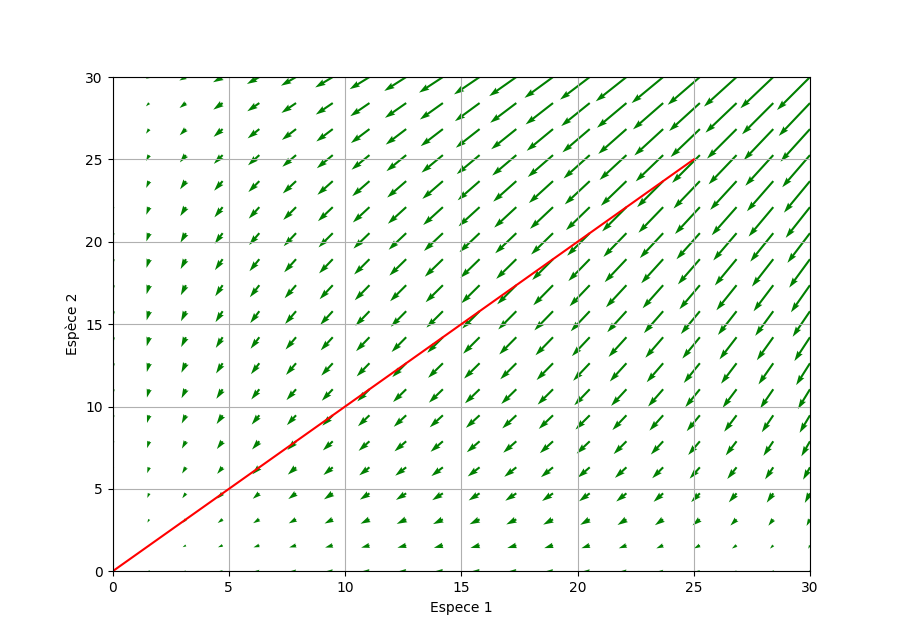
\includegraphics[scale = 0.6]{point (0,0).png}
    \caption{Extinction rapide des deux espèces}
    \label{1}
\end{figure}

\begin{tabular}{c|c}
     $r_1$&-2  \\
     \hline
     $r_2$&-2 \\
     \hline
     $K_1$&30 \\
     \hline
     $K_2$&30\\
     \hline
     $\alpha$&-1\\
     \hline
     $\beta$&-1\\
     \hline
     Cond. Init& $(25,25)$
\end{tabular}
\end{center}


Avec les paramètres choisis pour cette situation où$r_1$ et $r_2$ sont négatif, nous pouvons observer que le nombre d'individus de chacune des deux espèces devient nul au bout d'un certain temps et il le reste.\\\\

Pour le couple $(K_1,0)$ les valeurs propres sont $-r_1$ et $r_2$($1-\cfrac{\beta K_1}{K_2}$). Si ces deux valeurs sont négatives (comme c'est le cas dans la figure ci-dessous), alors le point $(K_1,0)$ est asymptotiquement stable; c'est un point de convergence du portrait de phase, comme c'est le cas ci-dessous: \\
\begin{center}

\begin{figure}[H]
    \centering
    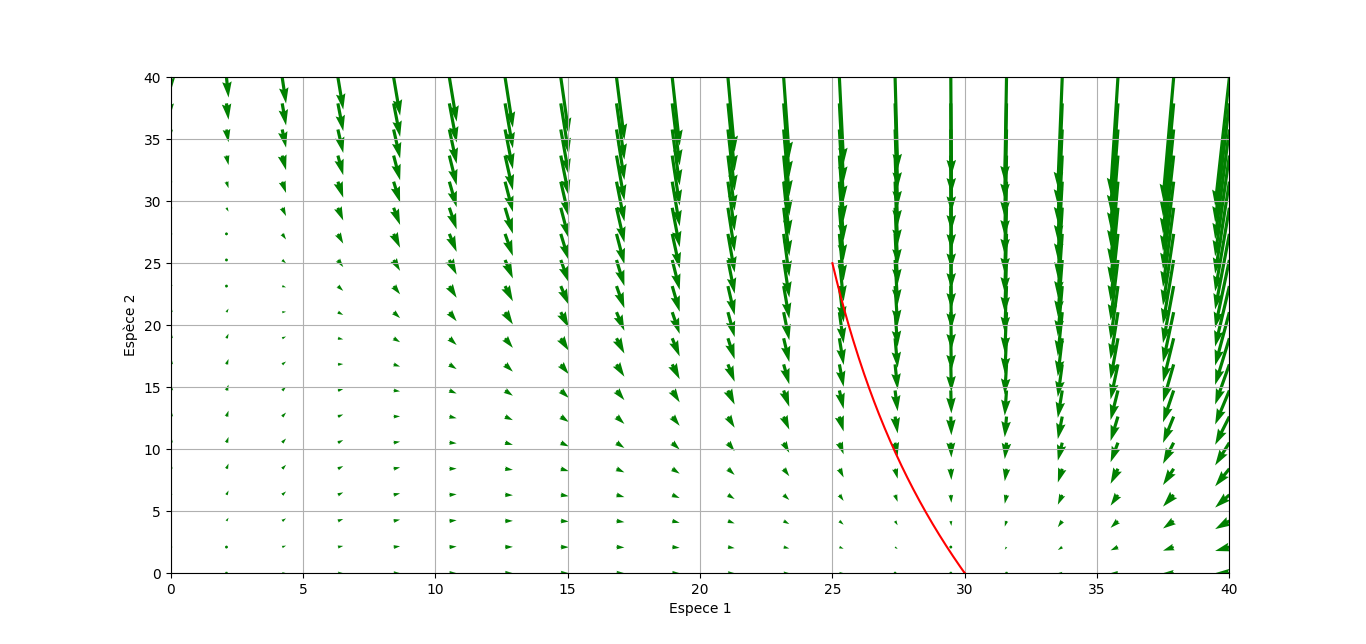
\includegraphics[scale = 0.4]{point(K1,0).png}
    \caption{Extinction de la deuxième espèce et maintien de la première à $K_1$}
    \label{1}
\end{figure}
\begin{tabular}{c|c}
     $r_1$&1  \\
     \hline
     $r_2$&1 \\
     \hline
     $K_1$&30 \\
     \hline
     $K_2$&30\\
     \hline
     $\alpha$&0\\
     \hline
     $\beta$&2\\
     \hline
     Cond. Init& $(25,25)$
\end{tabular}
\end{center}

Ici, la première espèce a une influence positive en valeur mais négative dans les faits sur la seconde alors que la deuxième espèce n'a pas d'influence sur la première. Le résultat est logique : au bout d'un certain temps l'espèce 2 s'éteint à cause de l'influence négative que l'espèce 1 exerce. L'espèce 1 se stabilise au nombre d'individus que le milieu peut naturellement nourrir.\\

Pour le couple $(0,K_2)$ les valeurs propres sont $-r_2$ et $r_1$($1-\cfrac{\alpha K_2}{K_1}$). Si ces deux valeurs sont négatives (comme c'est le cas dans la figure ci-dessous), alors le point $(0,K_2)$ est asymptotiquement stable.
\begin{center}

\begin{figure}[H]
    \centering
    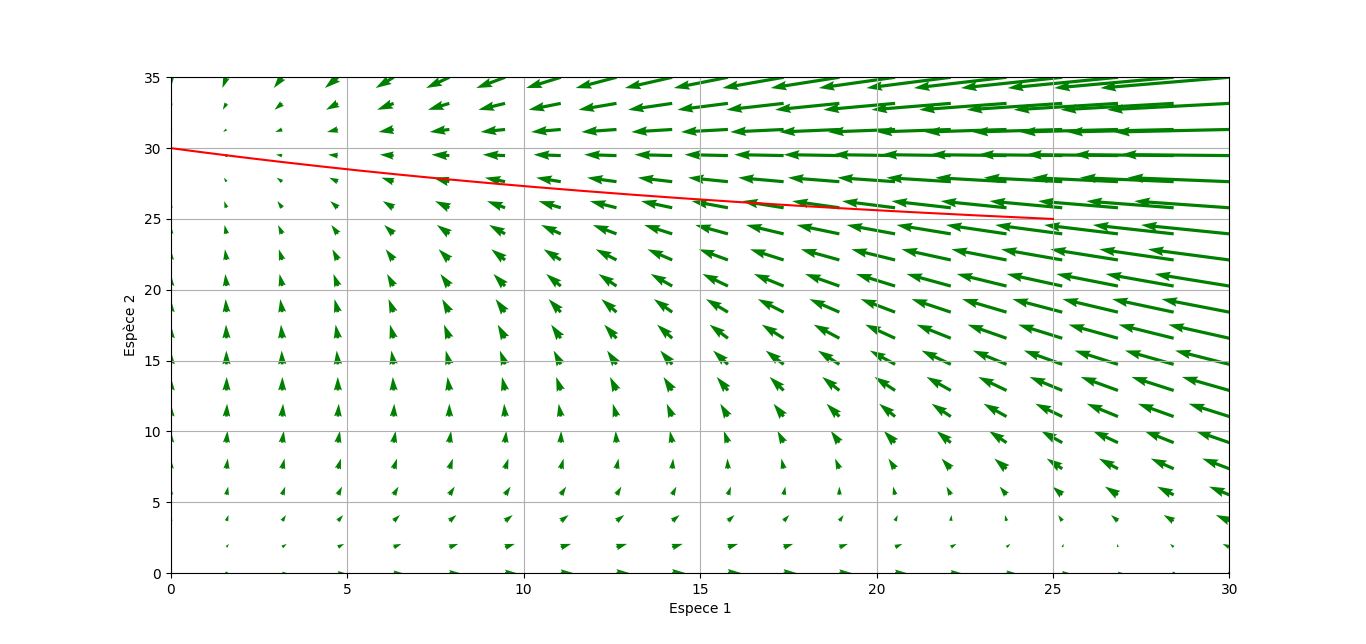
\includegraphics[scale = 0.4]{point(0,K2).png}
    \caption{extinction de la première espèce et maintien de la deuxième à $K_2$}
    \label{1}
\end{figure}
\begin{tabular}{c|c}
     $r_1$&1  \\
     \hline
     $r_2$&1 \\
     \hline
     $K_1$&30 \\
     \hline
     $K_2$&30\\
     \hline
     $\alpha$&2\\
     \hline
     $\beta$&0\\
     \hline
     Cond. Init& $(25,25)$
\end{tabular}
\end{center}


Ici, la deuxième espèce a une influence négative égale à 2 sur la première alors que la première espèce n'a pas d'influence sur la deuxième. Le résultat est logique: à un certain moment l'espèce 1 s'éteint à cause de l'influence que l'espèce 2. L'espèce 2 se stabilise au nombre que d'individu que le milieu peut naturellement nourrir.\\\\

Quand on étudie les valeurs propres associés à la matrice jacobienne du point\\
$(K_1 - \alpha \dfrac{K_2-\beta K_1}{1 -\alpha \beta},\dfrac{K_2-\beta K_1}{1 -\alpha \beta})$  on trouve ces deux valeurs:
$\lambda_1$ = $\dfrac{-n_1r_1}{K_1}$ et $\lambda_2$ = $\dfrac{-n_2r_2}{K_2}$

Avec $n_1 = K_1 - \alpha \dfrac{K_2-\beta K_1}{1 -\alpha \beta}$ et $ n_2 = \dfrac{K_2-\beta K_1}{1 -\alpha \beta}$\\

Nous pouvons en conclure que si $\dfrac{n_1r_1}{K_1}$ et $\dfrac{n_2r_2}{K_2}$ sont positif, $\lambda_1$ et $\lambda_2$ sont négatives, donc $(K_1 - \alpha \dfrac{K_2-\beta K_1}{1 -\alpha \beta},\dfrac{K_2-\beta K_1}{1 -\alpha \beta})$ est asymptotiquement stable et peut-être un point de convergence de notre fonction. Voyons un exemple qui satisfait ces conditions:
\begin{center}

\begin{figure}[H]
    \centering
    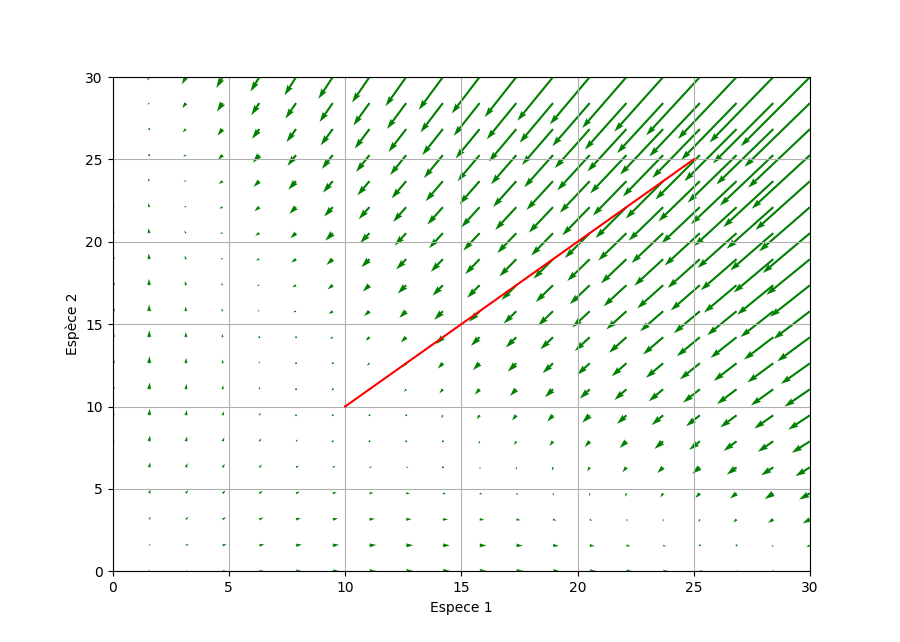
\includegraphics[scale = 0.55]{point(K1-...,...).png}
    \caption{Convergence vers notre point}
    \label{1}
\end{figure}

\begin{tabular}{c|c}
     $r_1$&1  \\
     \hline
     $r_2$&1 \\
     \hline
     $K_1$&30 \\
     \hline
     $K_2$&30\\
     \hline
     $\alpha$&2\\
     \hline
     $\beta$&2\\
     \hline
     Cond. Init& $(25,25)$
\end{tabular}
\end{center}

Ici, le point $(K_1 - \alpha \dfrac{K_2-\beta K_1}{1 -\alpha \beta},\dfrac{K_2-\beta K_1}{1 -\alpha \beta})$ est égal à (10,10). On a bien $n_1$, $n_2$, $r_1$, $r_2$, $K_1$, $K_2$ strictement positifs. $\lambda_1$ et $\lambda_2$ sont donc négatives. Ce point est donc asymptotiquement stable et on observe qu'il est bien point de convergence dans notre cas; les deux espèces se stabilisent à 10 individus. Cela semble logique puisque les deux espèces ont exactement les mêmes paramètres. On peut imaginer que comme les deux espèces exerce toutes les deux une influence égale l'une sur l'autre, elles se mettent la pression simultanément pour se stabiliser à 10 individus chacune au lieu des 25 du départ.

\subsubsection{Un système particulier : Cohabitation de deux espèces}
\begin{center}

\begin{figure}[H]
    \centering
    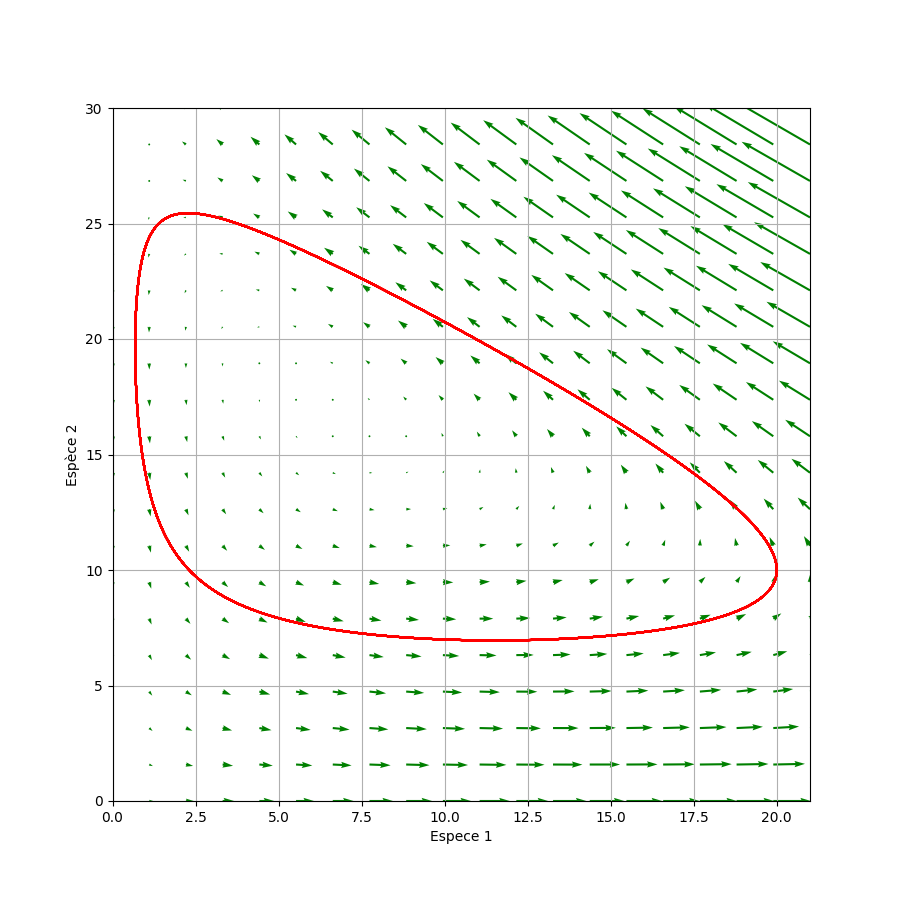
\includegraphics[scale = 0.42]{proiepreda.png}
    \caption{Assimilation à un système Proie-Prédateurs}
    \label{1}
\end{figure}

\begin{tabular}{c|c}
     $r_1$&2  \\
     \hline
     $r_2$&-0.6 \\
     \hline
     $K_1$&40 \\
     \hline
     $K_2$&30\\
     \hline
     $\alpha$&2\\
     \hline
     $\beta$&2\\
     \hline
     Cond. Init& $(20,10)$
\end{tabular}
\end{center}

Pour modéliser ce système et l'apparenter à un système proie-prédateurs nous avons dû réfléchir à comment combiner les différentes constantes. La première espèce a un taux de croissance positif et possède une influence positive sur la seconde. On peut prendre par exemple des lapins qui sont capables de survivre seuls dans une forêt et qui sont bénéfiques pour des loups. La seconde espèce, les loups ont un taux de croissance négatif, en effet sans lapins ils vont s'éteindre et disparaître. Leur influence est négative sur les lapins. La combinaison de tous ces facteurs entraîne une périodicité des populations.

Les deux populations semblent trouver un équilibre mais il n'y a pas de convergence ! Quand on regarde tous les couples de valeurs propres associées aux point d'équilibre de notre exemple, au moins une des deux est positive: il n'y a donc pas de point asymptotiquement stable.


\subsection{Espèces en compétitions : $\alpha,\beta \ne 0$ \& $\gamma,\delta \ne 0$ }
$\gamma$ et $\delta$ sont des facteurs de conversion, ils prennent des valeurs comprises entre -1 et 1. Ces facteurs permettent de renforcer les interactions entre les deux espèces. 
\begin{center}
\begin{math}
J = 
\begin{pmatrix} 
r_1 - \cfrac{2r_1N_1}{K_1} - \cfrac{\alpha r_1N_2}{K_1} + \gamma N_2 & - \cfrac{\alpha r_1N_1}{K_1} + \gamma N_1 \\
- \cfrac{\beta r_2N_2}{K_2} - \delta N_2   & r_2 - \cfrac{2r_2N_2}{K_2} - \cfrac{\beta r_2N_1}{K_2} - \delta N_1  \\
\end{pmatrix}
\end{math}
\end{center}

Nous allons calculer les points d'équilibres du système puis étudier s'ils sont stables ou non.
\newline

Les points d'équilibres sont $(0,0)$,$(K_1,0),(0,K_2)$ et le point ci-dessous
\begin{center}
$\Bigg(\dfrac{K_{1}+(\dfrac{\gamma r_{1}}{K_{1}}-\alpha)K_{2}}{1+(\dfrac{\gamma r_{1}}{K_{1}}-\alpha)(\dfrac{\delta r_{2}}{K_{2}}+\beta)},
K_{2}-\dfrac{K_{1}+(\dfrac{\gamma r_{1}}{K_{1}}-\alpha)K_{2}}{\dfrac{K_{2}}{\delta r_{2}+\beta K_{2}}+(\dfrac{\gamma r_{1}}{K_{1}}-\alpha)}\Bigg)$.
\end{center}
%% Je ne sais pas quels sont les paramètres que l'on peut fixer ici car tous les paramètres sont non nuls
%% du coup il y a plusieurs cas à faire
%%je pense qu'il est impossible de voir tous les cas possibles
%% il serait mieux de se mettre d'accord sur ce qu'on veut montré et le reste (certain) on les mettra en amélioration
Le couple $(0,0)$ a déjà été traité plus haut.\\

Pour le couple $(K_1,0)$ : les valeurs propres sont $-r_{1}$ et $r_{2}-\dfrac{\beta r_{2}K_{1}}{K_{2}}-\delta K_{1}$\\

Pour le couple $(0,K_{2})$ : les valeurs propres sont $-r_{2}$ et $r_{1}-\dfrac{\alpha r_{1}K_{2}}{K_{1}}+\gamma K_{2}$\\


Pour le dernier couple, nous n'avons pas calculé les valeurs propres de la jacobienne car le calcul est très compliqué. Nous dirons simplement que ce dernier point est soit stable et attractif ou instable en fonction de la valeur des paramètres.



\section{Améliorations du modèle}
Premièrement, ce système ne modélise que 2 espèces dans un environnement mais dans la nature, dans l'océan par exemple, des dizaines d'espèces cohabitent formant un véritable réseau alimentaire complexe. Il est ainsi possible de complexifier ce système en ajoutant une ligne par nouvelle espèce de la façon suivante : 
\begin{center}
\[ \dfrac{dN_i}{dt} = r_iN_i\Big(1 - \dfrac{\sum\limits_{j=1}^R \alpha_{ij}N_j}{K_i}\Big) \]
\end{center}

Deuxièmement, lors de nos différents tests, nous avons constaté qu'une espèce s'éteignait si et seulement si sa population est nulle. Dans la réalité, on sait qu'une espèce avec un nombre d'individus très limité est condamnée à s'éteindre. En effet, pour rester pérenne une espèce doit posséder une population suffisante pour ne pas subir les effets des tares génétiques et doit pouvoir résister à une vague de décès due à l'environnement. Il faudrait donc rajouter des conditions au système qui font converger vers 0 la population d'une espèce trop peu nombreuse.


\section{Conclusion}
Pour conclure, nous avons étudié les équations de compétitions de Lotka-Volterra en les complexifiant peu à peu à l'aide de nouveaux paramètres. Ce système nous a permis de modéliser le comportement  de deux populations avec plus ou moins d'interactions entre elles et constater quels étaient les effets de ces interactions. A travers nos tests, nous avons pu observer les différentes limites de ce modèle qui s'avère à la fois complexe mais également simple sur certains aspects.
Nous avons également vérifié la théorie des points d'équilibres grâce à la résolution des équations différentielles à l'aide d'un code Python orienté objet. En effet, les travaux pratiques effectués au préalable en cours de Python nous ont permis d'acquérir les connaissances nécessaires pour mettre en place un code efficace et réutilisable. Celui-ci ne se limite donc pas uniquement au modèle étudié. Il peut facilement être réutilisé et réadapté à un autre modèle.

Au début de l'étude du modèle, nous ne savions pas de quel côté l'aborder. Nous avons débuté avec méthode en commençant par une analyse mathématique au lieu de se lancer bille en tête et tester des paramètres au hasard. Cette étape de réflexion nous a permis de mieux saisir les tenants et les aboutissants du problème afin de continuer le TP sereinement.
\end{document}